\documentclass[12pt]{article}
\usepackage{latexsym,amssymb,amsmath} % for \Box, \mathbb, split, etc.
% \usepackage[]{showkeys} % shows label names
\usepackage{cite} % sorts citation numbers appropriately
\usepackage{path}
\usepackage{url}
\usepackage{verbatim}
\usepackage[pdftex]{graphicx}

% horizontal margins: 1.0 + 6.5 + 1.0 = 8.5
\setlength{\oddsidemargin}{0.0in}
\setlength{\textwidth}{6.5in}
% vertical margins: 1.0 + 9.0 + 1.0 = 11.0
\setlength{\topmargin}{0.0in}
\setlength{\headheight}{12pt}
\setlength{\headsep}{13pt}
\setlength{\textheight}{625pt}
\setlength{\footskip}{24pt}

\renewcommand{\textfraction}{0.10}
\renewcommand{\topfraction}{0.85}
\renewcommand{\bottomfraction}{0.85}
\renewcommand{\floatpagefraction}{0.90}

\usepackage{accents}
\newcommand{\ubar}[1]{\underaccent{\bar}{#1}}
\makeatletter
\setlength{\arraycolsep}{2\p@} % make spaces around "=" in eqnarray smaller
\makeatother
\usepackage{stackengine}
% change equation, table, figure numbers to be counted inside a section:
\numberwithin{equation}{section}
\numberwithin{table}{section}
\numberwithin{figure}{section}

% begin of personal macros
\newcommand{\half}{{\textstyle \frac{1}{2}}}
\newcommand{\eps}{\varepsilon}
\newcommand{\myth}{\vartheta}
\newcommand{\myphi}{\varphi}

\newcommand{\IN}{\mathbb{N}}
\newcommand{\IZ}{\mathbb{Z}}
\newcommand{\IQ}{\mathbb{Q}}
\newcommand{\IR}{\mathbb{R}}
\newcommand{\IC}{\mathbb{C}}
\newcommand{\Real}[1]{\mathrm{Re}\left({#1}\right)}
\newcommand{\Imag}[1]{\mathrm{Im}\left({#1}\right)}
\DeclareRobustCommand{\brkbinom}{\genfrac[]{0pt}{}}
\newcommand{\norm}[2]{\|{#1}\|_{{}_{#2}}}
\newcommand{\abs}[1]{\left|{#1}\right|}
\newcommand{\ip}[2]{\left\langle {#1}, {#2} \right\rangle}
\newcommand{\der}[2]{\frac{\partial {#1}}{\partial {#2}}}
\newcommand{\dder}[2]{\frac{\partial^2 {#1}}{\partial {#2}^2}}
\usepackage{enumitem}
\newcommand{\nn}{\mathbf{n}}
\newcommand{\xx}{\mathbf{x}}
\newcommand{\uu}{\mathbf{u}}
\usepackage{tikz}
\usetikzlibrary{arrows}
\usetikzlibrary{positioning}
\usepackage{titlesec}
\newcommand{\junk}[1]{{}}
\usepackage{sectsty}
\usepackage{xcolor}
\newcommand*{\bfrac}[2]{\genfrac{}{}{0pt}{}{#1}{#2}}
\newcommand\myatop[2]{\left[{{#1}\atop#2}\right]} % "wrapper macro"
\usepackage{array}
\usepackage{multirow}
\usepackage{amsmath}
\DeclareMathOperator*{\argmax}{arg\,max}
\DeclareMathOperator*{\argmin}{arg\,min}
\makeatletter
\renewcommand*\env@matrix[1][\arraystretch]{%
	\edef\arraystretch{#1}%
	\hskip -\arraycolsep
	\let\@ifnextchar\new@ifnextchar
	\array{*\c@MaxMatrixCols c}}
\makeatother

\makeatletter
\renewcommand*\env@matrix[1][*\c@MaxMatrixCols c]{%
	\hskip -\arraycolsep
	\let\@ifnextchar\new@ifnextchar
	\array{#1}}
\makeatother

\definecolor{darkblue}{rgb}{0,0,0.4}
\usepackage[colorlinks = true,
linkcolor = darkblue,
urlcolor  = darkblue,
citecolor = darkblue,
anchorcolor = darkblue]{hyperref}
% set two lengths for the includegraphics commands used to import the plots:
\newlength{\fwtwo} \setlength{\fwtwo}{0.45\textwidth}
% end of personal macros

\begin{document}
\DeclareGraphicsExtensions{.jpg}

\begin{center}
\textsc{\Large Statistical Pattern Recognition} \\[2pt]
	\textsc{\large Assignment 3}\\
	\vspace{0.5cm}
  Ali Gholami \\[6pt]
  Department of Computer Engineering \& Information Technology\\
  Amirkabir University of Technology  \\[6pt]
  \def\UrlFont{\em}
  \url{https://aligholamee.github.io}\\
    \href{mailto:aligholami7596@gmail.com}{\textit{aligholami7596@gmail.com}}
\end{center}

\begin{abstract}
In this paper, we'll review the \textit{parametric} techniques to estimate the \textit{unknown} parameters of data distributions. We'll use, \textit{MLE} and \textit{Bayesian} estimation for \textit{parameter estimation}. Also, we'll delve into the \textit{non-parametric} techniques to estimate the unknown \textit{density} of data distribution. We'll use \textit{Kernel Density Estimation} methods such as \textit{Parzen Windows} and other techniques such as \textit{Histogram} and \textit{k-NN} density estimation.
\end{abstract}

\subparagraph{Keywords.} \textit{Parameter Estimation, Density Estimation, Non-parametric Methods, Parametric Methods, Kernel Density Estimation, Maximum Likelihood Estimation, Bayesian Estimation, Histogram Density Estimation, K-NN Density Estimation.}

\section{General Maximum Likelihood Estimation}
Let ${x_k}$, $k = 1, 2, ..., N$ denote independent training samples from one of the following densities. Obtain the Maximum Likelihood estimate of $\theta$ in each case.
\begin{enumerate}[label=(\alph*)]
	\item $ f(x_k;\theta) = \frac{x_k}{\theta^2}\exp(\frac{-x_k^2}{2\theta^2}) $ where $x_k \geq 0$ and $\theta \ge 0$
	\item $ f(x_k;\theta) = \sqrt{\theta}x_k^{\sqrt{\theta} - 1}$ where $0 \leq x_k \leq 1$ and $ \theta \ge 0$
\end{enumerate}
\subsection*{Solution}
(a) Substituting the given density inside the \textit{MLE} equation yields the following results.
\begin{equation}
	\hat{\theta} = \text{arg}\,\max\limits_{\theta}\, \{P(D|\theta)\} = \text{arg}\,\max\limits_{\theta}\, \{\sum_{k = 1}^{n} \ln P(x_k|\theta)\} 
\end{equation}
$$
	\hat{\theta} = \text{arg}\,\max\limits_{\theta}\, \{\sum_{k = 1}^{n} \ln \frac{x_k}{\theta^2}\exp(\frac{-x_k^2}{2\theta^2})\}
$$
$$
	\nabla_{\theta}l(\theta) = 0 
$$
where $l(\theta)$ is $\sum_{k = 1}^{n} \ln \frac{x_k}{\theta^2}\exp(\frac{-x_k^2}{2\theta^2})$ in this case. Performing the gradient on the given equation yields the following results.
$$
	\sum_{k = 1}^{n} (\frac{-2}{\theta} + \frac{x_k^2}{\theta^3}) = 0
$$
The simplified estimate of unknown $\theta$ is given below.
$$
	\hat{\theta} = \sqrt{\frac{\sum_{k = 1}^{n} x_k^2}{2N}}
$$
(b) Substituting the given density in the Maximum Likelihood method yields the following result.
\begin{equation}
	\hat{\theta} = \text{arg}\,\max\limits_{\theta}\, \{\sum_{k = 1}^{n} \ln \sqrt{\theta}x_k^{\sqrt{\theta} - 1}\}
\end{equation}
we can obtain the estimate for the unknown $\theta$:
$$
	\nabla_{\theta}l(\theta) = 0 
$$
where $l(\theta)$ is $\sum_{k = 1}^{n} \ln \sqrt{\theta}x_k^{\sqrt{\theta} - 1}$ in this case. Performing the gradient on the given equation yields the following results.
$$
	\frac{n}{2\theta} + \frac{1}{2\sqrt{\theta}\sum_{k = 1}^{n}\ln x_k} = 0
$$
multiplying the whole equation by $\theta$ results in the following equation:
$$
	\hat{\theta} = \frac{n^2}{(\sum_{k = 1}^{n}\ln x_k)^2}
$$

\section{Uniform Maximum Likelihood Estimation}
Let $x$ have a uniform density

	\[ f_x(x|\theta) \sim U(0, \theta) = 
	\begin{cases}
	\frac{1}{\theta}       & \quad 0 \leq x \leq 0\\
	0  & \quad otherwise
	\end{cases}
	\]
	
\begin{enumerate}[label=(\alph*)]
	\item Suppose that n samples $ D = {x_1, x_2, ..., x_n}$ are drawn independently according to $f_x(x|\theta)$. Show that the maximum likelihood estimate for $\theta$ is $max[D]$.
	\item Suppose that n = 5 points are drawn from the distribution and the maximum value of which happens to be $max{x_k} = 0.6$. Plot the likelihood $f_x(D|\theta)$ in the range $0 \leq \theta \leq 1$. Explain in words why you do not need to know the values of the other four points.
\end{enumerate}
\subsection*{Solution}
(a) Substituting the uniform density function in the Maximum Likelihood method yields the following results.
\begin{equation}
\hat{\theta} = \text{arg}\,\max\limits_{\theta}\, \{\sum_{k = 1}^{n} \ln \frac{1}{\theta}\}
\end{equation}
This equation can be written as
$$
	\hat{\theta} = \text{arg}\,\max\limits_{\theta}\, \{l(\theta)\}
$$
where $l(\theta) = \sum_{k = 1}^{n} \ln \frac{1}{\theta}$. Performing a gradient on $l(\theta)$ would give us the Maximum Likelihood Estimate of $\theta$.
$$
	\sum_{k = 1}^{n} \frac{-1}{\theta} = 0 \rightarrow \frac{n}{\theta} = 0
$$
thus 
$$
	\hat{\theta} \rightarrow \inf
$$
Since $\hat{\theta} \rightarrow \inf$ and $\hat{\theta}\  \epsilon\  \{x_1, x_2, ..., x_n\}$ we'll have:
$$
	\hat{\theta} = max[D]
$$
(b) Since $	\hat{\theta} = max[D] $ we can simply plot the diagram as following.
\begin{figure}[!h]\centering
	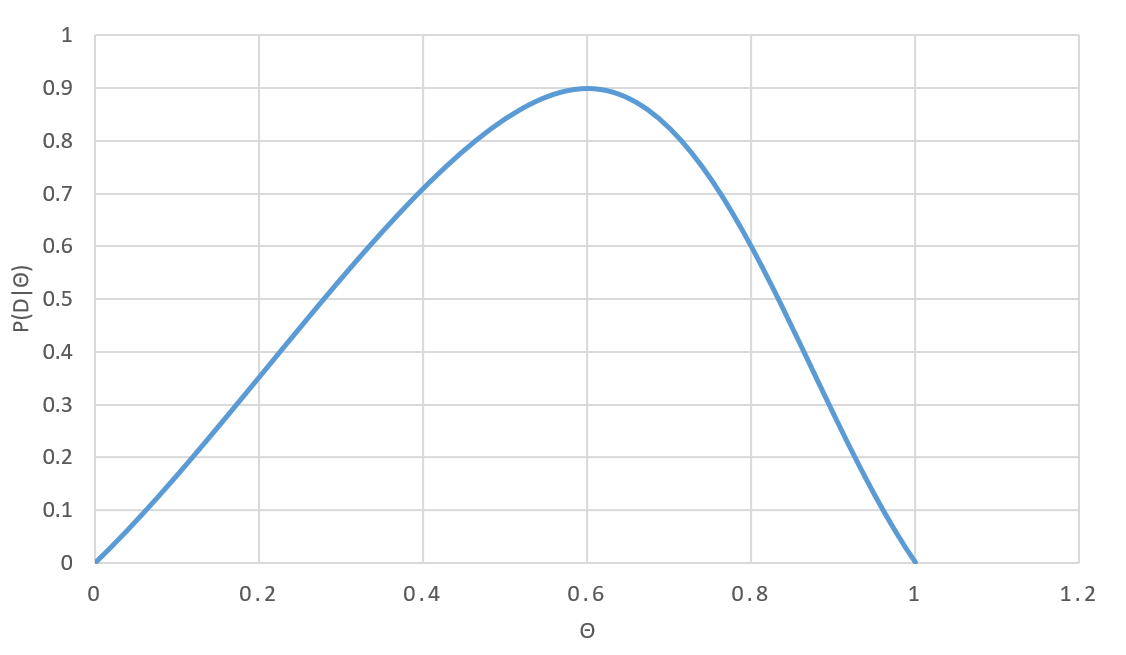
\includegraphics[width=0.8\textwidth]{2_b.PNG}
	\caption{Maximum Likelihood Estimation of $\theta$.}
	\label{pl1}
\end{figure}

The other four points wouldn't have maximized the likelihood $P(D|\theta)$.
\section{Density Estimation; Histogram, Parzen Windows and K-NN Method}
In this section, we'll be implementing top non-parametric methods for density estimation. We've implemented the 1-D and 2-D Scenario of density estimation in the \textit{src} folder. The experiment results are provided here.
\subsection*{Histogram Density Estimation}
\subsubsection*{Core Definition}
In this method, we'll divide the range of available samples to multiple bins. Then we'll count the number of samples in each bin. Let $k_i$ be the number of sample in $i$th bin and $V$ the size of bins($V = h^d$ where $h$ is the size of the bin in each dimension). The density for the $i$th bin can be estimated using the following formula. $n$ is the number of total samples.
\begin{equation}
	\hat{p}_{(x)} = \frac{k}{n * V}
\end{equation}
\subsubsection*{Python Implementation}
Full implementation with guiding comments can be found in \textit{src} folder. Note that in this implementation i've not used the internal bindings for kernel density estimation of Sklearn.
\begin{itemize}
	\item (1-Dimensional) | ($\mu = 5$) | ($var = 3$) | ($bin = 2$) | ($|D| = 100$)
	\begin{figure}[!h]\centering
		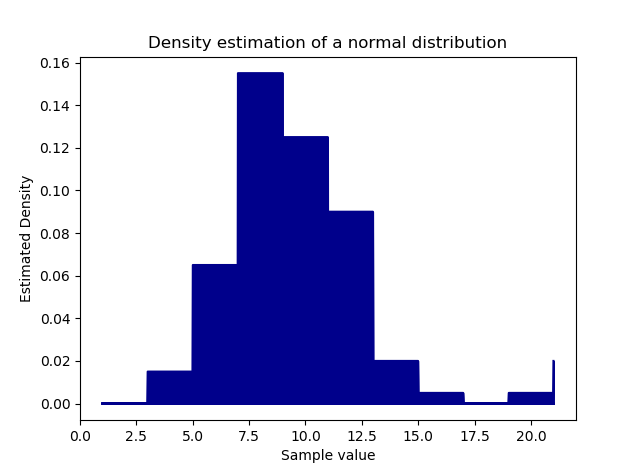
\includegraphics[width=0.6\textwidth]{3_a_1.PNG}
		\caption{1-D Histogram Density Estimation | Bin Size = 2}
		\label{pl1}
	\end{figure}
	
	\item (2-Dimensional) | ($\mu = 	\begin{bmatrix}
	8 & 8\\
	\end{bmatrix}$) | ($var = 	\begin{bmatrix}
	2 & 0\\
	0 & 2\\
	\end{bmatrix}$) | ($bin = 1$) | ($|D| = 5000$)
	\begin{figure}[!h]\centering
		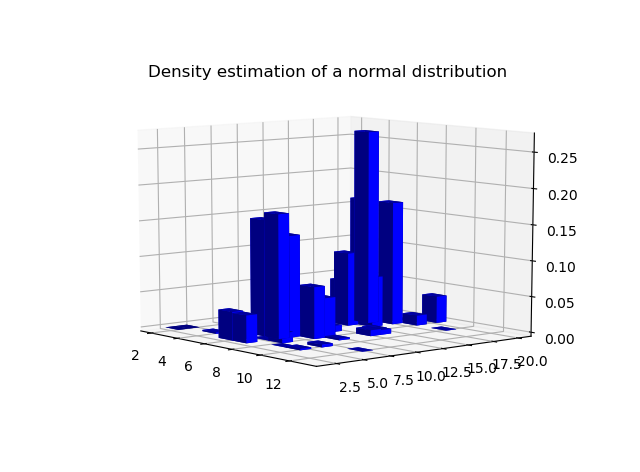
\includegraphics[width=0.8\textwidth]{3_a_2.PNG}
		\caption{2-D Histogram Density Estimation.}
		\label{pl1}
	\end{figure}
	
\end{itemize}
\subsubsection*{Bin Size Selection Analysis}
The results in figure 3.1 was given with a bin size of $2$. Smaller bin size result in a sharp and spiky estimation. However, choosing a bigger bin size results in an smoother estimation. As an example, figure 3.3 and 3.4 illustrates this phenomenon.
	\begin{figure}[!h]\centering
	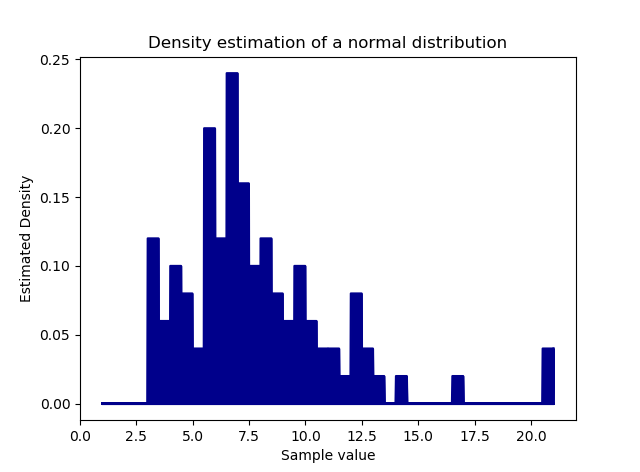
\includegraphics[width=0.8\textwidth]{3_a_3.PNG}
	\caption{1-D Histogram Density Estimation | Bin Size = 0.5}
	\label{pl1}
\end{figure}

	\begin{figure}[!h]\centering
	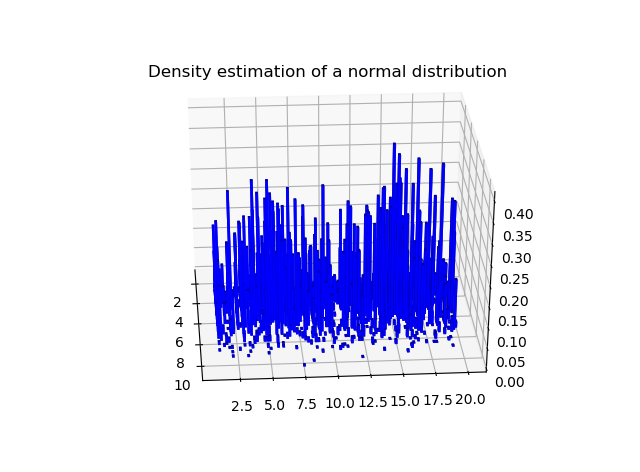
\includegraphics[width=0.8\textwidth]{3_a_4.PNG}
	\caption{2-D Histogram Density Estimation | Bin Size = 0.2 | Increased Sample Size}
	\label{pl1}
\end{figure}
\subsection*{Density Estimation with Parzen Windows(KDE)}
\subsubsection*{Core Definition}
In the method, each of the kernels are represented by $\Phi(x)$. These kernels will be placed on every single sample derived from the main distribution and the estimated density will be represented as following. In this equation, the $k$ stands for the number of samples we have derived from the main distribution. $h$ is called \textit{Bandwidth} and $h^d$ illustrates the Parzen window in a $d$ dimensional space.
\begin{equation}
	\hat{p}_{(x)} = \frac{1}{n*h^d} \sum_{i = 1}^{k}\Phi(\frac{x - x_i}{h})
\end{equation}
\subsubsection*{Python Implementation}
This section is implemented using \textit{Numpy, Matplotlib} and \textit{Scipy}. The gray density illustrates the distribution of our data and the blue one represents the estimate using Gaussian windows.
	\begin{figure}[!h]\centering
	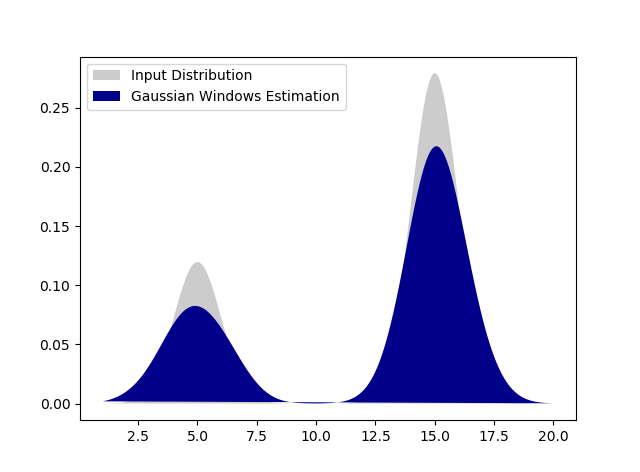
\includegraphics[width=0.8\textwidth]{3_b_1.PNG}
	\caption{1-D Multi-modal Gaussian Density Estimation using Gaussian Kernels.}
	\label{pl1}
\end{figure}

	\begin{figure}[!h]\centering
	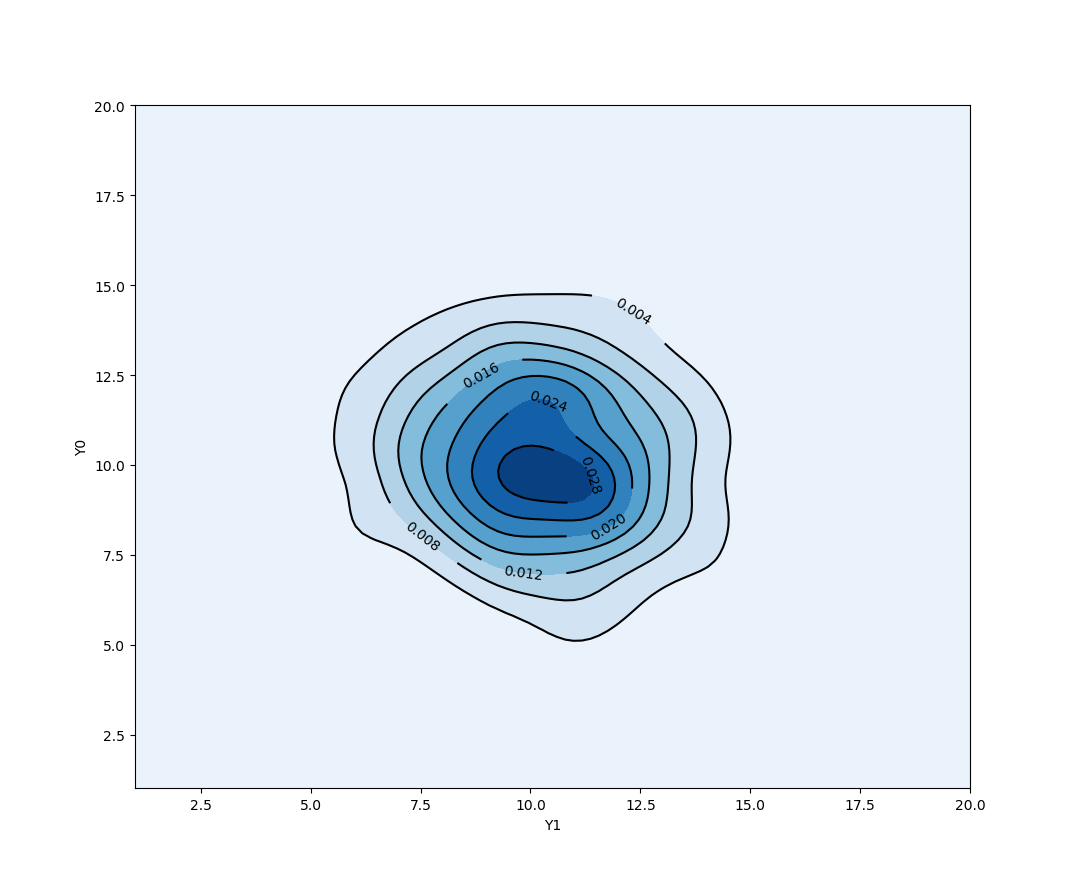
\includegraphics[width=0.8\textwidth]{3_b_2.PNG}
	\caption{2-D Gaussian Density Estimation using Gaussian Kernels | Bandwidth = 0.9}
	\label{pl1}
\end{figure}
\subsubsection*{Bandwidth Selection Analysis}
The results in figure 3.6 is given with a bin size of $0.9$. Smaller bandwidths result in a sharp and spiky estimation. However, choosing a bigger bandwidth results in an smoother estimation. As an example, figure 3.7 and 3.8 illustrates this phenomenon.
	\begin{figure}[!h]\centering
	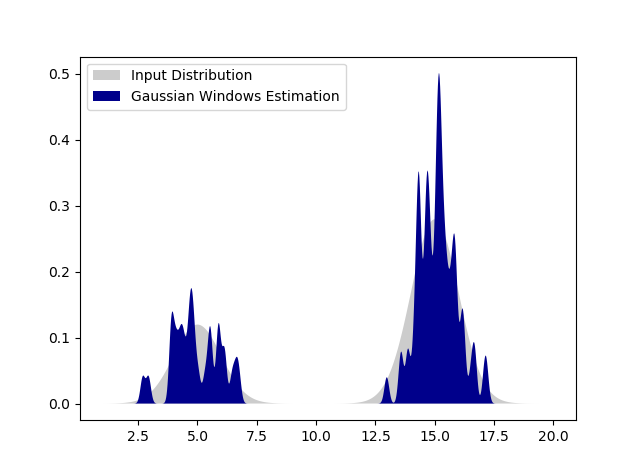
\includegraphics[width=0.8\textwidth]{3_b_3.PNG}
	\caption{1-D Multi-modal Gaussian Density Estimation using Gaussian Kernel | Bandwidth = 0.1}
	\label{pl1}
\end{figure}

	\begin{figure}[!h]\centering
	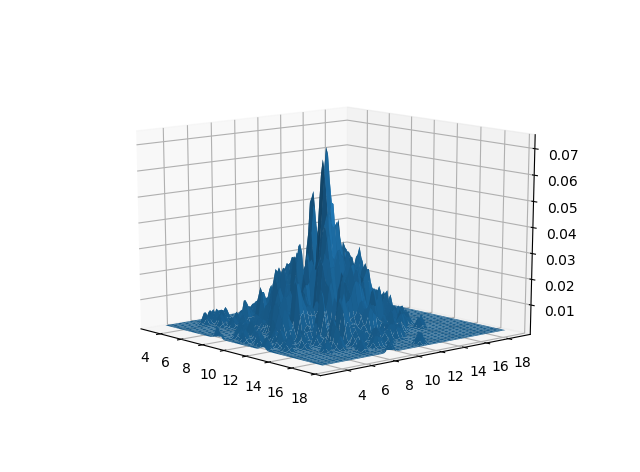
\includegraphics[width=0.8\textwidth]{3_b_4.PNG}
	\caption{2-D Gaussian Density Estimation using Gaussian Kernels | Bandwidth = 0.2}
	\label{pl1}
\end{figure}

\end{document} 

